\documentclass[a4paper,12pt]{article}
\usepackage{enumerate}

%% Language and font encodings
\usepackage[english]{babel}
\usepackage[utf8x]{inputenc}
\usepackage[T1]{fontenc}

%% Sets page size and margins
\usepackage[a4paper,top=3cm,bottom=2cm,left=1.5in,right=1in,marginparwidth=1.75cm]{geometry}

%% Useful packages
\usepackage{amsmath}
\usepackage{graphicx}
\usepackage{tikz}
\usepackage[colorinlistoftodos]{todonotes}
\usepackage[colorlinks=true, allcolors=blue]{hyperref}
\usepackage{dsfont}
\usepackage[document]{ragged2e}
\usepackage{titlesec}
\usepackage{mdframed}
\usepackage{amssymb}

\usepackage[justification=centering,format=plain,font=it]{caption}
\usepackage{minted}
\usepackage{setspace}

\usetikzlibrary{shapes}

%\newcommand{\sectionbreak}{\clearpage}
\newtheorem{theorem}{Theorem}
\newtheorem{lemma}[theorem]{Lemma}
\newtheorem{invariant}[theorem]{Invariant}

\setlength{\parskip}{1em}
%\titleformat{\section}[block]{\color{blue}\Large\bfseries\filcenter}{}{0.5em}{}

\title{Functionally Verified B+ Trees}
\author{Brian McSwiggen\\
        Advised by Professor Andrew Appel}

\begin{document}
\maketitle

\clearpage

\doublespacing

\section{Abstract}

In this thesis, I make progress toward a fully verified functional B+\,tree program in Coq. A verified functional B+\,tree would serve as the basis for the future verification of an imperative B+\,tree program through proving equivalence, which would have applications in databases and other systems. The primary focus of the properties and abstractions in this thesis is to examine and describe the theory of the B+\,tree cursor, which is central to the operations of a B+\,tree both functionally and imperatively. The functional implementation presented here covers the essential cursor operations as well as B+\,tree lookups and insertions, but does not include a delete function. The progress made toward verification includes the development of a complete abstract specification, the structural correctness of cursor creation and positioning, and the relation of cursors and B+\,tree operations to an element-list abstract cursor representation.

\clearpage

\section{Introduction and Motivation}

B+\,trees are an extension of the more commonly known B-trees, which are N-ary trees often used to organize data in file systems. The property that makes B+\,trees unique is that the \textit{values}, that is the data actually being held in the tree, are kept exclusively at the leaves. The interior nodes hold only keys and pointers to their children.

One interesting consequence of this property is that B+\,trees in practice can be augmented with a linked list between the leaf nodes connecting all of the values. This makes finding a value stored in the tree efficient (due to the tree structure) while still keeping range queries and iteration over the values easy (due to the linked list). Additionally, because B+\,trees don’t have to store as much data in the interior nodes, a single node can fit more pointers, meaning that the fanout can be larger and the tree needs fewer levels, so data can be accessed more quickly \cite{elmasri_navathe_2011}. A well-designed B+\,tree will store enough values per leaf that a single leaf node just fits into a single storage block, allowing the maximum possible amount of data retrieval with the fewest possible I/O operations.

Because this is a data structure commonly used by databases and file systems \cite{elmasri_navathe_2011}, it is a critical component underlying a great portion of the systems and software we rely on every day. On the one hand, that means that B+\,tree implementations used in practice are likely to be very well tested; on the other hand, bugs or failures have the potential to be wide-reaching and catastrophic.

That risk of failure is why rigorous testing practices are widely recognized as crucial to making good software that works correctly. However, in the most critical cases, more certainty may be necessary. The development of “formal methods” has provided an option for a greater degree of confidence in a range of critical applications. Formal methods encompass a range of approaches to applying strict mathematical rigor to software and hardware design, and “formal verification” in particular is the practice of rigorously proving algorithmic correctness. Because of the high certainty attained through formal methods, they have been applied to three categories of software: safety-critical, security-critical, and systems-critical programs.

Safety-critical software (or hardware) is a category of systems with direct impact on human life and safety. For example, if an airplane processor fails, if a nuclear reactor control has a bug, or if a defibrillator misfires, the consequences could very likely include death or serious injury. For that reason, software development for these systems has sometimes turned to formal methods to ensure correctness. In one example from as far back as the 1970s, NASA commissioned an aircraft control computer called SIFT which was subject to very strict failure-rate limits. Formal verification was used to ensure that the SIFT software for using redundant systems to detect and recover from hardware failures would work correctly \cite{225554}.

Security-critical software, while it does not always carry the same risk to human life, does carry the risk of compromising crucial cryptographic tools, data privacy and integrity, and more. Much such software is incredibly important to modern technology, but is also very intricate, hard to implement correctly, and hard to keep secure. Formal verification provides a means of reasoning about these tricky tools. In 2015, the Verified Software Toolchain group completed a full verification of an OpenSSL HMAC implementation, meaning that as long as SHA-256 is in fact cryptographically secure (which remains unproven), the HMAC is as well \cite{190894}.

Systems-critical software carries a great amount of risk because many other systems and pieces of software rely on it. While it may not itself carry risk to human life, or to cryptographic security, if any safety-critical or security-critical software runs on a system then it carries that risk indirectly. This has led a push to develop fully verified system stacks, such as the CLInc stack of compiler, assembler, kernel, and microprocessor, which were all verified correct in the 1980s \cite{225554}. A more relevant example to this project is the Verified Software Toolchain developed by Andrew Appel at Princeton, which also includes the CompCert verified C-language compiler developed by Xavier Leroy at INRIA \cite{Leroy:2009:FVR:1538788.1538814}.

Because of the many systems that directly or indirectly depend on B+\,trees, the verification of such an implementation falls under the systems-critical category. Formally proving a B+\,tree implementation correct increases our trust in the storage systems we use underneath any other piece of software, including any safety- or security-critical applications that may be built on top.

\clearpage

\section{Previous Work}

Formal verification is a rich field of study, and a large body of research has focused both on verifying software and on tools to make the verification of software easier. Search trees, as an important and complex class of data structures, have been the subject of previous verification. Recent work at Princeton and other universities has focused on the science and tools of specification and verification.

Various interesting search tree variants, in both functional\footnote{\textit{Functional} programming refers to a programming paradigm by which execution is the evaluation of a mathematical function, and all data are immutable (i.e. there is no program state). Well-known functional programming languages include Haskell, Lisp, and OCaml.} and imperative\footnote{\textit{Imperative} programming refers to a programming paradigm by which state-based programs are built up from individual statements, or commands. Well-known imperative programming languages include C, Java, and Python.} languages, have been the subject of verification work. An educational specification and proof of basic binary search trees can be found in Verified Functional Algorithms \cite{appel} by Professor Andrew Appel of Princeton University, who also published an efficient verified functional implementation of Red-Black trees in 2011 \cite{appel_2011}. Appel’s paper in turn builds upon the work of Filliâtre and Letouzey in 2004, in which they verified functional implementations of finite sets in three ways: using ordered lists, AVL trees, and Red-Black trees \cite{filliatre:hal-00150913}. This paper was a powerful demonstration of the use of Coq modules to contain both definitions and proven properties about those definitions, and this approach has been used here as well in the abstract specification.

Functional program verification such as the work done by Appel, Filliâtre, and Letouzey serves a practical purpose both because it can help find bugs in current functional libraries (as Filliâtre and Letouzey did with the OCaml Set module based on AVL trees \cite{filliatre:hal-00150913}) and because it can be extracted from Coq into live OCaml code and used in practice. However, many practical applications rely on imperative software. As an example in the domain of search trees, Xiwen Chen of York University provided a verified concurrent imperative binary search tree which he had proven linearizable, i.e. that any operation performs correctly as if it executed immediately \cite{chen_ruppert_breugel_2013}. Although it is more difficult to reason about imperative programs than about purely functional ones, doing imperative verifications is crucial for practical application of formal verification.

There are many approaches and tools which have been developed and can be used to reason about imperative software. Although this thesis focuses on the verification of a purely functional program, such a functional verification can serve as a crucial intermediate step in proving properties of an imperative program. The functional B+\,trees discussed here will be used to ultimately prove correctness of a B+\,tree implementation written in C. The tools and techniques that will be used for the \textit{imperative} proof provide a framework for what a useful \textit{functional} B+\,tree verification is, and are described in the following sections.

\subsection{Separation Logic}

A group at Princeton University and the National University of Singapore very recently included a demonstration of a verified binary search tree as part of a paper on separation logic and the “magic wand” connective (separating implication) \cite{cao_wang_hobor_appel_2017}. \textit{Separation logic} is a set of logic rules extending Hoare logic that facilitate proofs about variably sized imperative data structures (such as arrays or trees) by allowing the program state to be separated into disjoint parts about which properties can be proven \cite{1029817}.

Separation logic is crucial because having to reason about the entirety of the program state together quickly gets very complicated. On top of the desired properties, there have to be assertions for exactly what parts of the program state any given command affects, and assertions that no other part of the program is affected, and assertions that any two portions of a program intended to be affected differently are in fact disjoint \cite{1029817}. It is easy to see how the whole structure does not scale well within Hoare logic, which is why separation logic is so important for the verification of many imperative programs.

\subsection{Verified Software Toolchain}

\begin{figure}[h]
    \begin{center}
		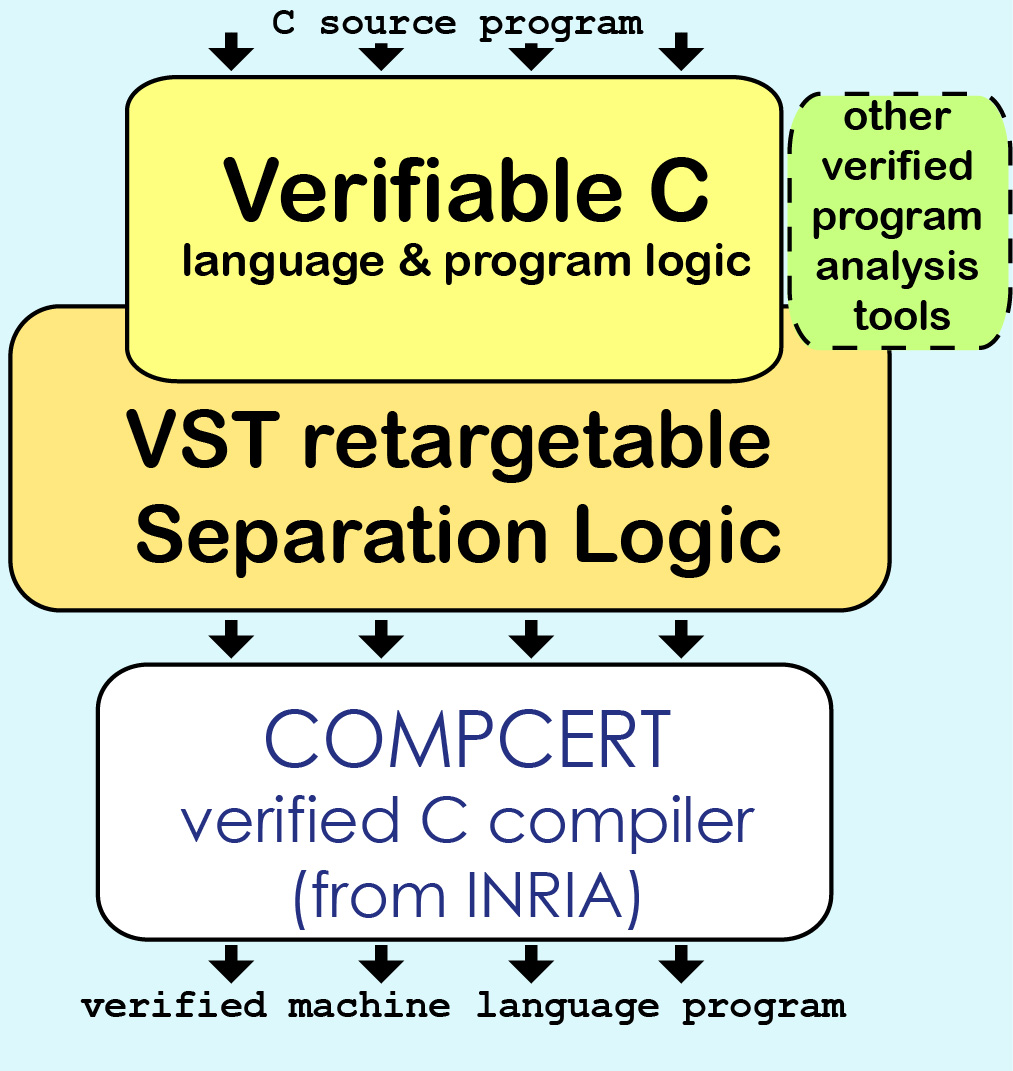
\includegraphics[]{b}
        \caption{Diagram of VST components \protect\cite{vst_2017}}
    \end{center}
\end{figure}

Separation logic is crucial not just to a proof about a particular program, such as our B+\,trees implementation, but also to the entire verification stack that it is based on. Since the mid-2000s, a group at Princeton University led by Professor Andrew Appel has been developing the \textit{Verified Software Toolchain} \cite{vst_2017}, a stack of verified components that allow proofs to be written about source programs and apply to the compiled program as well. Each component of the toolchain, from the Verifiable C program logic to Xavier Leroy’s CompCert C compiler to the machine language operational semantics (and all of the interfaces between them), is designed for verification and proven correct \cite{10.1007/978-3-642-19718-5_1}.

Although the scope of this thesis does not extend into connecting the B+\,tree specification to an imperative C program that it represents, the functional specification produced could be useful for the verification of a C program. The strategy of functional specification used in this thesis is intended to work with the Verified Software Toolchain, so that a C program could be proven via the VST separation logic to be equivalent to this functional specification.

\subsection{DeepSpec}

The Verified Software Toolchain itself is part of a larger research group called DeepSpec. Since 2016, the DeepSpec group at Princeton, University of Pennsylvania, Yale, and MIT have been collaborating under an NSF Expedition in Computing grant to explore the science of deep specifications. This thesis is in part an attempt to extend that work by applying deep specification to a B+\,tree database program. Deep specifications, as described by the DeepSpec group, are program specifications with four special properties \cite{deepspec}:

\begin{enumerate}
\item They are \textbf{rich}, that is, they can describe the complex behavior of real programs.
 
\item They are \textbf{two-sided}. Specifications function analogously to interfaces in modular programming: they describe the boundary between two independent parts. A two-sided specification is one that is exercised from both sides of the boundary, i.e. it matches both the program it describes and the programs that use it.

\item They are \textbf{formal}, meaning they are written in exact mathematical terms. Specifications that are provided only as vague or intuitive definitions may have holes or errors that are hard to spot. Formal specifications can be machine-checked and tested.

\item They are \textbf{live}, that is, they are connected directly to the implementation and the client code. If either changes, then the machine-checked proofs may no longer pass; this ensures that when the proofs are verified we can be sure they describe the actual program.
\end{enumerate}

In the course of their work, the DeepSpec group and their collaborators are developing an extensive network of systems-related programs connected at deep specification interfaces. The goal is to be able to construct a verified stack from the operating system and applications like the B+\,tree database all the way down to the machine language and transistors at the core of the computer.

The previously mentioned Verified Software Toolchain being developed by Appel is one part of this stack. It also includes a verified LLVM (VeLLVM) developed by Steve Zcancewic at UPenn, a verified operating system (CertiKOS) developed by Zhong Shao at Yale, and many other tools, systems, and applications.

\clearpage

\section{Project Approach and Scope}

The strategy that this thesis targets for verifying imperative software is through a \textit{functional model}. A functional model describes the actual behavior of the operations, and in this case the model is an equivalent piece of software written in a functional programming language, but other functional models are possible. When reasoning about a programming language, for example, the functional model might be the small-step operational semantics of the language. For the purposes of this thesis, since functional programs are much easier to formally reason about, the functional model provides a bridge: we can prove the equivalence of the functional program and the imperative program, and then any proofs of correctness for the functional program are also valid proofs of the imperative one.

One step beyond the functional model is the \textit{abstract specification}. This describes, in the most pure and abstract terms possible, the goal for the program. The abstract specification defines what it \textit{means} to be a “correct implementation” of the desired program. Proving these properties of the functional model proves that the model is correct, and therefore any imperative program equivalent to the model is also correct.

The scope of this thesis covers a B+\,tree abstract specification, a functional implementation, and a partially formalized proof of the implementation’s correctness relative to the specification. Once completely formally verified, the functional program could be used as the functional model for an imperative program, but that step is not covered in this work. 

The particular style of B+\,tree and set of operations which are targeted in this work are derived from a subset of the SQLite commands. SQLite uses B+\,trees to store information in relational databases. One particularity of SQLite is that it represents a cursor into the B+\,tree as a list of pointers to the split point at each level. This makes it easier to change the position of the cursor without needing to have a linked list at the leaves as mentioned above or having to retraverse the tree.

\clearpage

\section{B+ Tree Details} \label{sec:b+tree}

A B+\,tree is a type of ordered tree with three important properties:

\begin{enumerate}
\item Any B+\,tree has a \textit{max fanout} value $b$ which represents the maximum number of children that any node can hold. Every node in the B+\,tree except the root must have between $\lceil \frac{b}{2} \rceil$ and $b$ children; the root may have as few as two (if it is an interior node) or one (if it is a leaf node) \cite{elmasri_navathe_2011}.

\item All \textit{values} are stored in leaf nodes. Interior nodes only store keys and pointers to the child nodes. This means that an interior node with $n$ children only needs to store $n-1$ keys, and also that keys may repeat in the tree \cite{elmasri_navathe_2011}.

\item As new key-value pairs are inserted, the tree only grows up at the root, not down at the leaves: when a node gets too big and splits, both halves become children of the original parent node, and no new levels are added to the tree. The only way for a new level to be added is for the root node to split and create a new root node above it. Similarly, as key-value pairs are deleted, the tree shrinks at the root rather than at the leaves. This ensures that the whole tree always stays balanced, that is, the distance from any leaf to the root is the same as the distance from any other leaf to the root \cite{elmasri_navathe_2011}.
\end{enumerate}

An interior node in a B+\,tree might look like the following:

%Maybe come back and clean this up later%
\begin{table}[h]
\centering
\begin{tabular}{|l|l|l|l|l|l|l|}
\hline
$P_1$ & $K_1$ & $P_2$ & $K_2$ & ... & $K_{n-1}$ & $P_n$\\
\hline
\end{tabular}
\caption{B+\,tree interior node with $n-1$ keys and $n$ subtrees}
\label{tab:interior-node}
\end{table}

Where each $P_i$ is a pointer to a child node, and each $K_i$ is a key. The fanout $n$ is constrained by $\lceil \frac{b}{2} \rceil \leq n \leq b$, the keys $K$ must be sorted ($ \forall i, j: \ K_i < K_j$), and each key $K$ constrains the values in the child nodes to either side: for every key $X$ in the node at $P_i, K_{i-1} \leq X < K_i$. Of course, for the end pointers, only one side of that inequality will hold \cite{elmasri_navathe_2011}.

A leaf node holds values rather than child pointers, and must have exactly one key per value. Therefore, a leaf node might look like the following:

%Maybe come back and clean this up later%
\begin{table}[h]
\centering
\begin{tabular}{|l|l|l|l|}
\hline
$(K_1,V_1)$ & $(K_2,V_2)$ & ... & $(K_n,V_n)$\\
\hline
\end{tabular}
\caption{B+\,tree leaf node with $n$ keys and $n$ values}
\label{tab:leaf-node}
\end{table}

In this case, each $V_i$ is some value stored by the B+\,tree (often, but not necessarily, a pointer to a block of data in memory), and each $K_i$ is once again a key. The keys must be sorted just as in the interior nodes, and it still holds that the fanout n is constrained by $\lceil \frac{b}{2} \rceil \leq n \leq b$ \cite{elmasri_navathe_2011}.

With this structure, we now consider how to do database operations on this structure. In particular, we describe Lookup (finding a key/value in a b+tree), Insert (adding a key/value pair), and Delete (removing a key/value pair).

For all three operations, we will consider the following b+tree for examples:

%Find a way to position better?%
%Find a way to italicize captions?%
\begin{figure}[h]
    \centering
    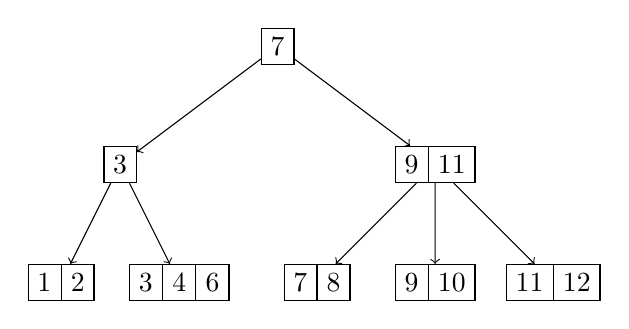
\begin{tikzpicture}
    \tikzstyle{bplus}=[rectangle split, rectangle split horizontal,rectangle split ignore empty parts,draw]
    \tikzstyle{every node}=[bplus]
    \tikzstyle{level 1}=[sibling distance=40mm]
    \tikzstyle{level 2}=[sibling distance=15mm]
    \node {7} [->]
      child {node {3}
        child {node {1 \nodepart{two} 2}}
        child {node {3 \nodepart{two} 4 \nodepart{three} 6}}    
      } 
      child {node {9 \nodepart{two} 11}
        child {node {7 \nodepart{two} 8}}
        child {node {9 \nodepart{two} 10}}   
        child {node {11 \nodepart{two} 12}}    
      }
    ;\end{tikzpicture}
    \caption{A simple B+\,tree of height 3. Each interior node has 2 or 3 children.}
    \label{fig:demotree1}
\end{figure}

Notice that all keys and subtrees are properly ordered, that all leaves are at depth 2 (where the root is depth 0), and that keys may appear multiple times within the tree. The fanout is $b=3$, meaning each node may have two or three children (this simple example is actually a variant of a 2-3 tree). For these examples, the values at the leaves have been left out, since they are irrelevant to the tree operations.

\subsection{Lookup}

Finding a key-value pair in the tree proceeds from the root. At each level, we search through the list of keys to find the split where the value we want falls. Since every node has a sorted list of keys, we can do binary search within a list if desired. However, the number of children is often small enough that a simpler linear search works as well, especially when the fanout is optimized for the size of CPU cache lines, rather than full disk pages.

If we were to search for 10 in the example tree, we would first note that $7 < 10$ and go to the second child of the root. We would then note that $9 \leq 10 < 11$, and go to the middle child, where we would find 10.

\begin{figure}[h]
    \centering
    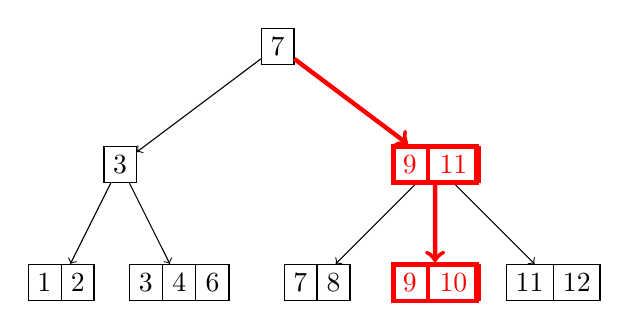
\begin{tikzpicture}
    \tikzstyle{bplus}=[rectangle split, rectangle split horizontal,rectangle split ignore empty parts,draw]
    \tikzstyle{every node}=[bplus]
    \tikzstyle{level 1}=[sibling distance=40mm]
    \tikzstyle{level 2}=[sibling distance=15mm]
    \node {7} [->]
      child {node {3}
        child {node {1 \nodepart{two} 2}}
        child {node {3 \nodepart{two} 4 \nodepart{three} 6}}    
      } 
      child[ultra thick,red] {node {9 \nodepart{two} 11}
        child[thin, black] {node {7 \nodepart{two} 8}}
        child[ultra thick, red] {node {9 \nodepart{two} 10}}   
        child[thin, black] {node {11 \nodepart{two} 12}}    
      }
    ;\end{tikzpicture}
    \caption{To find 10, we search for 10 at each level and recursively descend.}
    \label{fig:demotree2}
\end{figure}

\subsection{Insert}

Insertion is simple if the leaf node has less than $b$ children: we simply find the correct place according to the list of keys, and add the value there. However, we must maintain that any given node has at most b children. Therefore, if a key is inserted which would go into a leaf that has b children already, then we have to split that node and add the middle key to the node above \cite{elmasri_navathe_2011}.

If that node is also full, then we have to split it in turn, and so on up to the root where, if necessary, the root will split and the tree will grow by one level \cite{elmasri_navathe_2011}.

For a leaf node, since every key must appear mapped to its value, we keep the middle key in the leaf as well. However, for any interior node that splits, the middle key which goes up to the next level is removed from the level that split \cite{elmasri_navathe_2011}.

If we were to insert the key-value pair $(5,V_5)$ in the example tree, we would have to first find where in a leaf node 5 should go (between 4 and 6, on the left). Then, seeing that the leaf would have 4 key-value pairs, we split it in two and copy 5 up to the next level.

%Could use some work%
\begin{figure}[h]
    \centering
    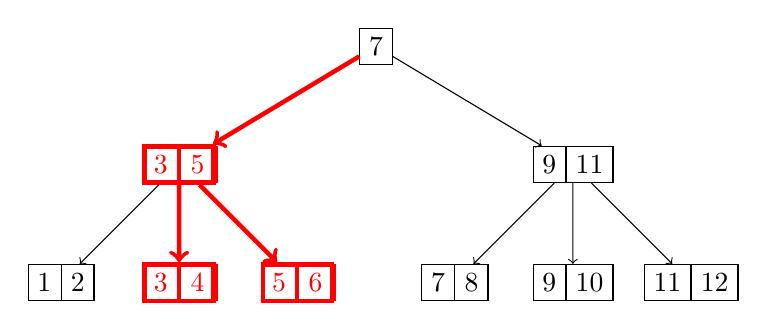
\begin{tikzpicture}
    \tikzstyle{bplus}=[rectangle split, rectangle split horizontal,rectangle split ignore empty parts,draw]
    \tikzstyle{every node}=[bplus]
    \tikzstyle{level 1}=[sibling distance=50mm]
    \tikzstyle{level 2}=[sibling distance=15mm]
    \node {7} [->]
      child[ultra thick,red] {node {3 \nodepart{two} 5}
        child[thin, black] {node {1 \nodepart{two} 2}}
        child[ultra thick, red] {node {3 \nodepart{two} 4}}
        child[ultra thick, red] {node {5 \nodepart{two} 6}}    
      } 
      child {node {9 \nodepart{two} 11}
        child {node {7 \nodepart{two} 8}}
        child {node {9 \nodepart{two} 10}}   
        child {node {11 \nodepart{two} 12}}    
      }
    ;\end{tikzpicture}
    \caption{To add a mapping for 5, we have to first find where 5 goes in the tree, then add the new key-value pair and split nodes as necessary.}
    \label{fig:demotree3}
\end{figure}

\subsection{Delete}

Deletion works intuitively as the inverse of insertion. It is simple if the leaf node has at least $\lceil \frac{b}{2} \rceil + 1$ entries; then we can just remove the entry and leave the rest of the tree as it is. However, if the leaf node would be left with less than $\lceil \frac{b}{2} \rceil$ entries after deletion, then we need to redistribute entries in order to maintain the fanout. That can happen by moving over entries from adjacent nodes (and changing the keys in the parent node), or by merging a node with adjacent nodes to reduce the total number of children. In the latter case, this reduction in the number of children may cause the parent to have to redistribute or merge as well, potentially propagating up to the root and decreasing the depth of the tree by one \cite{elmasri_navathe_2011}.

If we were to delete the key 9 from our example tree, we would see that its leaf now has only 1 entry. Since both adjacent nodes are too small to redistribute, we instead have to merge them.

\begin{figure}[h]
    \centering
    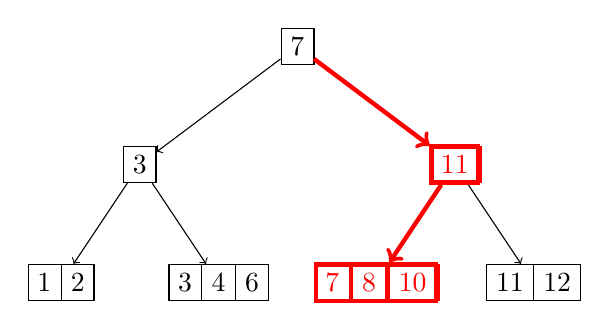
\begin{tikzpicture}
    \tikzstyle{bplus}=[rectangle split, rectangle split horizontal,rectangle split ignore empty parts,draw]
    \tikzstyle{every node}=[bplus]
    \tikzstyle{level 1}=[sibling distance=40mm]
    \tikzstyle{level 2}=[sibling distance=20mm]
    \node {7} [->]
      child {node {3}
        child {node {1 \nodepart{two} 2}}
        child {node {3 \nodepart{two} 4 \nodepart{three} 6}}    
      } 
      child[ultra thick,red] {node {11}
        child[ultra thick, red] {node {7 \nodepart{two} 8 \nodepart{three} 10}}
        child[thin, black] {node {11 \nodepart{two} 12}}    
      }
    ;\end{tikzpicture}
    \caption{When we delete 9, we may need to merge nodes together.}
    \label{fig:demotree4}
\end{figure}

\clearpage

\section{Abstract Specification} \label{sec:spec}

Our abstract specification of a B+\,tree is that of a lookup table. That is, it stores data indexed by keys, and allows that data to be arbitrarily fetched, changed, added to, or removed. However, we add one more layer to this particular table abstraction. B+\,trees rely on a cursor, which could be any way of pointing to a particular place in the table. We build this notion into our abstract specification, allowing us to prove correctness relative to this abstract notion of a cursor in addition to a table. Here, the specification is shown as written in Coq.

\begin{figure}[h]
\begin{singlespace}
\begin{minted}{coq}
Module Type CURSOR_TABLE.
 Parameter V: Type.
 Definition key := Z.
 Parameter table: Type.
 Parameter cursor: Type.
 Parameter empty_t: table.
\end{minted}
\end{singlespace}
\end{figure}

We parametrize our abstract cursor-table with a number of basic types. Any cursor-table must store a set of values of type \texttt{V}. It stores these within a table of type \texttt{table} (\texttt{empty\_t} being the most basic such table, storing no values) and accesses them using a cursor of type \texttt{cursor}. Any implementation of a cursor-table must provide these basic parameters, but the exact types are up to the specific implementation---this makes the module type abstract.

Notice that any cursor-table must also have a \texttt{key} type which is mapped to values. For our purposes we have hard-coded this as Coq’s built-in \texttt{Z} type for integers. Perhaps it would be better to abstract even further by allowing the key to be any type that has a compare function and satisfies some particular set of axioms; this was in fact the approach taken by Filliâtre and Letouzey in their verification of finite set implementations \cite{filliatre:hal-00150913}. However, the simplifying assumption that the keys will be integers is not an unreasonable one, and in particular it fits well with the imperative implementation that this functional specification could be used to verify.

\begin{figure}[h]
\begin{singlespace}
\begin{minted}{coq}
 Parameter make_cursor: key -> table -> cursor.
 Parameter get_table: cursor -> table.
 Parameter get_key: cursor -> option key.
 Parameter get: cursor -> option V.
 Parameter insert: cursor -> key -> V -> cursor.
 Parameter next: cursor -> cursor.
 Parameter prev: cursor -> cursor.
 Parameter first_cursor: table -> cursor.
 Parameter last_cursor: table -> cursor.
\end{minted}
\end{singlespace}
\end{figure}

Any cursor-table must also define a set of operations on the table. Again, the specific implementations are left abstract: they are constrained only by their type signatures and the required axioms about them discussed below.

The most central of these functions is the \texttt{make\_cursor} operation, which takes any key and a table and creates a cursor at the appropriate location for that key in the table. Such a cursor is then used as input to most other operations. The reverse of \texttt{make\_cursor} is \texttt{get\_table}, which translate from a cursor back into the table it points into. We also require two shortcuts for creating cursors at the extremes of a table, these are \texttt{first\_cursor} and \texttt{last\_cursor} and are important in the definition of later axioms.

Once we have set a cursor, a cursor-table should be able to use it to do any of the desired operations: \texttt{get} to retrieve the value stored at the cursor, \texttt{get\_key} to retrieve the key mapped to that value, and \texttt{insert} to update the tree with a new key-value pair. Deletion is not included as part of this specification, but could be axiomatized similarly to insertion.

The cursor should also be movable from its position: \texttt{next} should move it to the next key greater than the cursor’s current position, while \texttt{prev} should move it to the last key lesser than its current position.

\begin{figure}[h]
\begin{singlespace}
\begin{minted}{coq}
 Parameter abs_rel: table -> cursor -> Prop.
 Parameter key_rel: key -> cursor -> Prop.
 Parameter eq_cursor : cursor -> cursor -> Prop.
 Parameter cursor_correct: cursor -> Prop.
 Parameter table_correct: table -> Prop.
\end{minted}
\end{singlespace}
\end{figure}

We need various propositions that can describe the correctness and relationship of tables, cursors, and keys as well. Specifically, we need four propositions. The first, \texttt{abs\_rel}, defines what it means for a particular cursor to be a reference into a particular table, i.e. for the table and cursor to represent the same abstract relation. The second, \texttt{key\_rel}, defines what it means for a cursor to be positioned for a particular key $k$, i.e. that the key to the right of the cursor is greater than $k$ and the key to the left is at most $k$. The third, 
\texttt{eq\_cursor}, is a predicate for two cursors being abstractly equivalent even if they are not structurally equal. The fourth and fifth describe what it means for a cursor or table to be correct: since we don’t require every instance of the \texttt{cursor} and \texttt{table} types to be correct, it is possible to have a cursor or table that does not actually correspond to a valid instance of a \texttt{CURSOR\_TABLE}. For example, with B+\,trees it is possible to construct an unbalanced or unsorted tree, in which case the operations are not guaranteed to be correct. It would have been possible to make a more complicated B+\,tree type than the one described later in section \ref{sec:typedef} and enforce the correctness properties on every tree instance. However, this would have made working with that type more difficult.

\begin{figure}[h]
\begin{singlespace}
\begin{minted}{coq}
 Axiom make_cursor_rel: forall t k,
   abs_rel t (make_cursor k t).
 Axiom get_table_rel: forall t c,
   abs_rel t c <-> get_table c = t.
 Axiom first_rel: forall t,
   abs_rel t (first_cursor t).
 Axiom last_rel: forall t,
   abs_rel t (last_cursor t).
 Axiom next_rel: forall t c,
   abs_rel t c -> abs_rel t (next c).
 Axiom prev_rel: forall t c,
   abs_rel t c -> abs_rel t (prev c).
 Axiom correct_rel: forall t c,
   abs_rel t c -> (cursor_correct c <-> table_correct t).
\end{minted}
\end{singlespace}
\end{figure}

Given the above relations and propositions, we now want to ensure they satisfy certain desirable properties. \texttt{make\_cursor} and \texttt{get\_table} should function correctly relative to our table-cursor relation, as should \texttt{first\_cursor} and \texttt{last\_cursor}. Cursor repositioning (\texttt{next} and \texttt{prev}) should stay within the same table. Finally, correctness should translate between cursors and tables---if a cursor is correct, then so should its corresponding table be correct; and for any correct table, all cursors into that table should be correct.

\begin{figure}[h]
\begin{singlespace}
\begin{minted}{coq}
 Axiom insert_correct: forall k v c,
   cursor_correct c -> key_rel k c -> cursor_correct (insert c k v).
\end{minted}
\end{singlespace}
\end{figure}

Inserting a key-value pair into a correct cursor should in general return a new correct cursor. As a consequence of this, by \texttt{correct\_rel} and \texttt{get\_table\_rel} above, it also implies a new table (that is, \texttt{get\_table} of the new cursor) that is itself correct. However, notice that we add an additional restriction: the new cursor only has to be correct if it satisfies \texttt{key\_rel k c}, i.e. it was positioned properly for the key $k$ that was inserted. We don’t actually specify what should happen when inserting a key-value pair into a cursor in the wrong position. Depending on the implementation, it could work correctly, return the original cursor back unchanged (as our implementation does), or modify the cursor completely incorrectly. It doesn’t ultimately matter---we only require the behavior to be correct when the cursor is positioned correctly.

\begin{figure}[h]
\begin{singlespace}
\begin{minted}{coq}
 Axiom glast: forall t,
   get (last_cursor t) = None.
 Axiom gis: forall k v c,
   cursor_correct c -> key_rel k c ->
   get (make_cursor k (get_table (insert c k v))) = Some v.
 Axiom gio: forall j k v c,
   cursor_correct c -> key_rel k c -> ~ key_rel j c ->
   get (make_cursor j (get_table (insert c k v))) =
   get (make_cursor j (get_table c)).
\end{minted}
\end{singlespace}
\end{figure}

The next three axioms cover how \texttt{get} should behave. Specifically, we build up the behavior of \texttt{get} through modifications to the table. This reflects the idea that the behavior of \texttt{get} for a certain key should only be affected by certain modifications, and should ignore others. If we look up a particular key $k$ for which we have inserted some value $v$, we should get back that value $v$. On the other hand, if we look up a key $j$ into a table where we last inserted $k$, and $j$ and $k$ are not in the same range for the cursor $c$, then the behavior of \texttt{get} should be as if $k$ had never been inserted.

\begin{figure}[h]
\begin{singlespace}
\begin{minted}{coq}
 Axiom next_prev: forall c t,
   abs_rel t c -> ~ (c = last_cursor t) ->
   eq_cursor c (prev (next c)).
 Axiom prev_next: forall c t,
   abs_rel t c -> ~ (c = first_cursor t) ->
   eq_cursor c (next (prev c)).
 Axiom cursor_order: forall c k1 k2,
   cursor_correct c -> get_key c = Some k1 ->
   get_key (next c) = Some k2 -> lt_key k1 k2 = true.
End CURSOR_TABLE.
\end{minted}
\end{singlespace}
\end{figure}

Finally, we want to ensure that for any valid cursor except the last one, moving to the next position and then back to the first gives us back a cursor equivalent to the original; this is \texttt{next\_prev}. In the reverse direction, for any valid cursor except the first one, moving to the previous position and back gives us an equivalent cursor to the original cursor; this is \texttt{prev\_next}. Finally, we expect \texttt{next} and \texttt{prev} to position the cursor relative to the ordering of the table. If we call \texttt{next}, we expect the “next” key that it moves to to be the key immediately greater than the one the cursor was previously on.

Note that while all of these axioms do specify \textit{what} the cursor-table should do, they don’t specify \textit{how} it should do it. We implement this specification with B+\,trees, but it could as well be implemented with a simple binary tree, a linked list, an array, or many other data structures. That level of abstraction is crucial: we simplify our correctness properties to only the general results that we want to prove.

\subsection{A Small Example} \label{subsec:ex}

To demonstrate the application of the abstract specification as described above, consider a small example. Suppose we have a small relation built up by inserting $(3,V_3)$, then $(1,V_1)$, and finally $(2,V_2)$. Functionally, this might look like the following:

\begin{figure}[h]
\begin{singlespace}
\begin{minted}{coq}
insert (insert (insert (make_cursor 0 empty_t) 3 V_3) 1 V_1) 2 V_2
\end{minted}
\end{singlespace}
\end{figure}

Let the cursor returned by the final insert be $c$. If we now try to retrieve the value for key $1$ from $c$, we want to be able to prove that we get $V_1$ back. This might look like the following:

\begin{figure}[h]
\begin{singlespace}
\begin{minted}{coq}
get (make_cursor 1 (get_table c))
\end{minted}
\end{singlespace}
\end{figure}

If we peel off the outer \texttt{insert} of $c$, we see that we can apply \texttt{gio}:

\begin{figure}[h]
\begin{singlespace}
\begin{minted}{coq}
get (make_cursor 1 (get_table (insert c 2 V_2))) =
get (make_cursor 1 (get_table c))
\end{minted}
\end{singlespace}
\end{figure}

Peeling off the next \texttt{insert}, we can now apply \texttt{gis} and prove that we return $V_1$:

%For some reason the figure is making this mess up??
%\begin{figure}[h]
\begin{singlespace}
\begin{minted}{coq}
get (make_cursor 1 (get_table (insert c 1 V_1))) = Some V_1
\end{minted}
\end{singlespace}
%\end{figure}

In other words, without any knowledge of the specific implementation of any of the operations, and using only the theorems defined by the abstract specification, we have proved that the value returned by get is the intended value placed into the table.

\clearpage

\section{B+ Tree Type Specification} \label{sec:typedef}

The first step of writing an effective functional model is determining how to translate the imperative concepts of the B+\,tree data structure into functional terms. Pointers and mutable data have to be turned into immutable data that can be recursively destructed. In making decisions about how to design the functional type, we have to achieve two goals: first, creating a simple type that will be easy to prove correctness properties of, and second, creating a type that will be easy to prove equivalent to the imperative program.

\subsection{Tree Data Structure Type}

We represent a B+\,tree as a mutually inductive type of \texttt{tree} and \texttt{treelist}.

\begin{figure}[h]
\begin{singlespace}
\begin{minted}{coq}
Inductive tree : Type :=
 | node : key -> treelist -> tree
 | final : treelist -> tree
 | val : key -> V -> tree
with treelist : Type :=
 | tl_nil : treelist
 | tl_cons : tree -> treelist -> treelist
\end{minted}
\end{singlespace}
\end{figure}

Intuitively, \texttt{tree} holds the key-subtree mapping: each \textit{element} within a node is a tree. The \texttt{final} tree type holds the single subtree not paired with a key, since interior nodes have $n+1$ subtrees for $n$ keys. Then, an entire node is a \texttt{treelist}. An immediate similarity is apparent between the \texttt{treelist} type and Coq’s standard list type. This makes it convenient to destruct a treelist to iterate over it.

It also makes the single treelist type work for both interior nodes (which map keys to subtrees without values, and use the \texttt{node} and \texttt{final} tree types) and leaf nodes (which map keys to values, and use the \texttt{val} tree type). Since both of those nodes can be expressed by the single type \texttt{tree}, a treelist can hold either one. This in turn makes the structure of the B+\,tree simpler, but at the cost of added complexity and assumptions when proving properties of a tree. The type itself does not enforce the structural property that a node is \textit{either} a leaf node with \texttt{val}s or an interior node with \texttt{node}s and exactly one \texttt{final}, so we have to assume or prove this whenever needed.

The choice of putting a final tree at the end, rather than having an initial keyless subtree at the beginning, is somewhat out of sync with the imperative implementation. However, it makes both correctness proofs and the functional implementation much simpler.

Imagine that we had an initial keyless subtree at the beginning. We want to say that a treelist is structurally correct if it has exactly one keyless subtree. Once we destruct a correct treelist and remove that initial subtree, the remainder suddenly only has nodes, and is no longer structurally correct! By placing final at the end instead, a destructed treelist is still structurally correct.

Additionally, putting final at the end makes searching for a particular key (e.g. when making a cursor) easier. At each step, we need to compare the key we are looking for against the key for this subtree. With an initial keyless subtree, we would have to look at the key held in the \textit{next} tree at each step. With a final at the end, we only have to compare against the key held in the current node; once we get to final we know that any remaining keys have to be there.

When relating this representation to the imperative representation, it suffices to shift subtrees by one. In other words, the imperative implementation’s keyless “first pointer” is related to the first key’s subtree in the functional implementation; the imperative first key’s subtree is the functional second key’s subtree. The functional final subtree, which is keyless, is related to the imperative implementation’s last key’s subtree.

\subsection{B+ Tree Cursor Type}

Imperatively a cursor is a pointer to a particular entry in a B+\,tree. Once a cursor points to a part of a B+\,tree, it can be used to retrieve the value stored there, update it to store something else, or insert an entirely new key-value pair to the tree. In a functional B+\,tree there are no pointers per se, and we cannot update the tree in-place in the same way since all data is immutable. However, it is still useful to represent the idea of a cursor “pointing at” a particular position in a B+\,tree.

The representation used was to structure a pointer into a treelist as the combination of that treelist and the index of the cursor’s position within it. The \texttt{cursor} type is then a list of indices combined with a list of treelists. This cursor structure was chosen to make proofs more straightforward, because it contains the original tree structure unmodified, and the \texttt{make\_cursor} operation structurally matches the \texttt{treelist} type (this is explained in more detail in section \ref{subsec:cursorop}). However, other operations are slightly complicated because of the choice to use indices: every step requires destructing the treelist to find the right position before we can get or update the keys and values stored there.

\begin{figure}[h]
\begin{singlespace}
\begin{minted}{coq}
Definition cursor : Type := list nat * list treelist.
\end{minted}
\end{singlespace}
\end{figure}

Other possible representations of a cursor were also considered when designing the B+\,tree types for the functional model.\footnote{The primary other representation considered was to think of a cursor as a \textit{split} in a tree: it “points” to a particular part of the B+\,tree by actually separating it into the trees and treelists to the left of that part vs those to the right. The cursor type is then a list of treelist splits. Representing a cursor this way makes operations on that cursor simpler: getting the (key,value) pair at the cursor only requires looking at the entry immediately on the right in the first treelist split; updating it can be easily done by updating the value, gluing the split back together, and recursively inserting it back into the next level up. Unfortunately, this representation of a cursor complicates the task of cursor creation, and by consequence complicates the process of proofs about that cursor.} The choice of this particular representation was made to prioritize simplicity of proofs over simplicity of implementation. The purpose of this functional model is \textit{not} to be efficient---it exists as a tool to be proven about; with that in mind, it is almost always better to prioritize proofs over code when there is a trade-off to be made.

Note that this representation of a cursor is as a pair of \textit{lists} of individual treelist pointers. This might seem strange, since an imperative implementation only needs to store a single pointer to a single position. However, representing a cursor as a list of pointers reflects the structure of the SQLite cursor mentioned earlier, which is similarly a list of pointers to the relevant location at each level. It also greatly simplifies the functional implementation and proofs to be able to destruct and reconstruct the B+\,tree on a per-level basis, rather than needing to start from the root for any operation.

Also note that the \texttt{cursor} type as defined here has no way to distinguish between pointing \textit{at} an element versus pointing \textit{in between} two elements. In fact, in an abstract sense, a cursor is always considered to represent a split between two keys. In situations where we are considering the element that the cursor is on (e.g. when looking up a value), by default we assume it is the first element to the right of the cursor’s position. However, it is important to note that the cursor does not need to be on a particular element. For example, a cursor into an entirely empty table is completely valid, and is represented as any index into the treelist \texttt{tl\_nil}.

This adds a potential point for confusion: two \textit{structurally} different cursors could \textit{abstractly} represent the same split. Consider the following example:

%Do this%
---------Need a graphic for this---------

Both arrows represent the split between keys 2 and 6 in this B+\,tree---the first could be the result of \texttt{make\_cursor 3 f}, and the second the result of \texttt{make\_cursor 5 f}. Abstractly they are equivalent, and any operations on them should do the same thing. But in our implementation they are not actually equal structures. So we have to ensure (and prove) that all of our B+\,tree operations can detect this and treat it appropriately.

\clearpage

\section{Functional Implementation} \label{sec:func}

\subsection{Element-List Abstraction}

The question of proving that our B+\,tree operations treat cursors appropriately relies on an intuitive understanding of how cursors should behave that we now need to formalize. Within our implementation, a B+\,tree cursor is a list of indices and treelists. In the abstract specification, a B+\,tree cursor is only defined by how our operations use it. This leaves a gap in formalization that makes it difficult to prove our operations correct or prove that they use cursors appropriately.

To solve this problem, we introduce an intermediate abstraction of cursors as an element-list. An element, in this sense, is any key-value pair that appears in the B+\,tree. The tree itself then is a list of these elements in order by increasing key. A cursor splits that list into the parts before the cursor’s position and the parts after it, and to simplify our operations we reverse the order of the first list. In other words, the \textit{element-list abstraction} of a cursor is a pair of lists, one to the “left” and one to the “right”, where the first element in each list is the element immediately adjacent to the cursor on each side, and the last element in each list is the extreme first or last element of the tree.

It is clear that under this abstraction, functionally equivalent cursors are represented the same. If two structurally different cursors in the tree point to the same split, then they must have the same element-list abstraction. Furthermore, our operations on these element-lists are very simple. To lookup the value at a cursor, we simply pop an item off the right list and return its value. To insert a new key-value pair we just add it to the left list (placing the cursor just after it); to update the value for a key already in the list we just replace the value at the beginning of the right list. Moving the cursor position is just popping items off of one list and concatenating them to the other.

\subsection{Cursor Operations} \label{subsec:cursorop}

\begin{figure}[h]
\begin{singlespace}
\begin{minted}{coq}
Function make_cursor_rec (x: key) (f : treelist) (ci : list nat)
(ct : list treelist) (n : nat) : cursor :=
  match f with
  | tl_nil => (n::ci,ct)
  | tl_cons (node k f') f =>
    if lt_key k x then make_cursor_rec x f ci ct (S n)
    else make_cursor_rec x f' (n::ci) (f'::ct) O
  | tl_cons (final f') tl_nil =>
    make_cursor_rec x f' (n::ci) (f'::ct) O
  | tl_cons (val k v) f =>
    if lt_key k x then make_cursor_rec x f ci ct (S n)
    else (n::ci,ct)
  | _ => ([],[])
  end.

Definition make_cursor (x : key) (f : treelist) : cursor :=
  make_cursor_rec x f [] [f] O.
\end{minted}
\end{singlespace}
\end{figure}

Creating a cursor to point at a particular key $x$ happens in two stages. Within a particular treelist, we scan across each node, comparing the node’s key k against the target key x. This is what is happening in the \texttt{match} section: the treelist is decomposed horizontally into its component trees. As we scan across, we update a counter $n$ that represents the index within the treelist where the function currently is. Once we find the first key greater than or equal to $x$ (as in the \texttt{else} portion), we add that index onto the cursor that we are building and restart from 0 in the treelist below that index. If we ever hit a \texttt{final} tree, then we can assume this is the last tree in the treelist and descend into it without scanning the treelist further. For leaves, we will either hit a \texttt{val} that matches or we will hit \texttt{tl\_nil} because we have passed the end of the treelist. Either way, we can just append the index and return the cursor that has been built up.

Decomposing the creation of a cursor in this way helps to make induction and termination of this function easy. At each step we are destructing the treelist given and recursing on one of the two results. Since functional objects have no pointers and must be constructed from the data they hold, it is impossible to have an infinitely large tree, so it is easy for Coq to automatically prove the termination of this function. Similarly, when we are proving properties of \texttt{make\_cursor}, having a function that destructs the treelists naturally fits precisely with our induction scheme:

\begin{figure}[h]
\begin{singlespace}
\begin{minted}{coq}
treelist_tree_rec :
forall (P : tree -> Prop) (P0 : treelist -> Prop),
(forall (k : key) (t : treelist), P0 t -> P (node k t)) ->
(forall t : treelist, P0 t -> P (final t)) ->
(forall (k : key) (v : V), P (val k v)) ->
P0 tl_nil ->
(forall t : tree, P t ->
  forall t0 : treelist, P0 t0 -> P0 (tl_cons t t0)) ->
forall t : treelist, P0 t.
\end{minted}
\end{singlespace}
\caption{The induction scheme requires a property \texttt{P} that is inductively assumed about every tree, and a property \texttt{P0} that is assumed and proved about every treelist. Having functions destruct a treelist in both directions matches this scheme well.}
\label{fig:induction}
\end{figure}

This works well for making a cursor, but we still have the issue of multiple structurally distinct cursors which are abstractly the same. In order to do any operations with a cursor, we need a way to handle these two cursors equivalently. For this purpose, we wrote two normalization functions. The first, \texttt{next\_node}, normalizes a cursor so it points directly to a \texttt{val} tree; this would be the position pointed to by \texttt{make\_cursor 5} in the example tree from the previous section. The second, \texttt{prev\_node}, is the reverse: it normalizes a cursor so it has a val tree directly behind it, i.e. the \texttt{make\_cursor 3} position in the example tree. For both functions, the functions should change the structure of the cursor without changing the abstract element-list of the cursor.

\begin{figure}[h]
\begin{singlespace}
\begin{minted}{coq}
Fixpoint next_node (cn : list nat) (cf : list treelist)
: option (cursor * key) :=
  match (cn,cf) with
  | (n::cn',f::cf') =>
    (match point n f with
     | (_,Some (node k _),tl_cons (node _ f') _) =>
       Some (((S n)::cn',f::cf'),k)
     | (_,Some (node k _),tl_cons (final f') _) =>
       Some (((S n)::cn',f::cf'),k)
     | (_,Some (val k v), _) => Some ((n::cn',f::cf'),k)
     | _ =>
       (match next_node cn' cf' with
        | Some ((n'::cn,f'::cf),k) =>
          (match point n' f' with
           | (_,Some (node _ f1),_) =>
             Some ((O::n'::cn,f1::f'::cf),k)
           | (_,Some (final f1),_) =>
             Some ((O::n'::cn,f1::f'::cf),k)
           | _ => None
           end)
        | _ => None
        end)
     end)
  | (_,_) => None
  end.
\end{minted}
\end{singlespace}
\end{figure}

The central functionality of \texttt{next\_node} is to travel up the treelist as far as necessary to find a treelist that has a next tree to descend down into. It then positions itself before the very first element of that tree. If it is able to find such a modified cursor, it returns both that cursor and the pivot key at the highest node it reached (i.e., the key that separates the original cursor position from the new one). If it is not able to find such a cursor---in other words, if the cursor was already at the last possible position in the tree---then it returns \texttt{None}.

Here, \texttt{point n f} is a function that decomposes a treelist $f$ into three parts: the treelist before index $n$, the tree at index $n$ (if it exists, \texttt{None} otherwise), and the treelist after index $n$. We assume \texttt{next\_node} is called from a leaf node, so if there is a \texttt{val} that the cursor is already pointing to then we are done, and no modification is necessary. If there is something next to point to that is a \texttt{node} or a \texttt{final}, then we can assume we are in the middle of a recursive call. Since there is something next, this is the pivot tree, so we move the index up by one and attach the associated key $k$.

If we match \texttt{point n f} and find something else, for example \texttt{None} or a \texttt{final} tree, then we are at the end of a node and cannot point to the next thing. Therefore, we must recursively call \texttt{next\_node} to get the node adjacent to this one. Then we can move down into the tree pointed to by that partial cursor, and position a new (potentially partial) cursor at the first index of that tree.

The structure of \texttt{prev\_node} is very similar, but operating in reverse it destructs the cursor index to examine the tree immediately \textit{before} the cursor’s position. If it is at the beginning of a node and there is nothing directly preceding it to point to, then it recursively calls \texttt{prev\_node} at the next level up in the cursor. The partial cursor it gets back is then grown with the treelist $f’$ pointed to and a pointer to the last element of $f’$.

\begin{figure}[h]
\begin{singlespace}
\begin{minted}{coq}
Fixpoint move_to_next (c : cursor) : cursor :=
  match c with (cn,cf) =>
  (match next_node cn cf with
   | Some ((n::cn',cf'),_) => (S n::cn',cf')
   | _ => c
   end)
  end.

Fixpoint move_to_prev (c : cursor) : cursor :=
  match c with (cn,cf) =>
  (match prev_node cn cf with
   | Some ((S n::cn',cf'),_) => (n::cn',cf')
   | _ => c
   end)
  end.
\end{minted}
\end{singlespace}
\end{figure}

With these normalization functions, actually moving the cursor becomes trivial. We normalize to the next or prev position to ensure there is an adjacent element to move the cursor to, then we change the cursor to point to it.

Furthermore, the correctness of these functions follows directly from the correctness of the normalization functions. Given proofs that \texttt{next\_node} and \texttt{prev\_node} both produce correct cursors, then \texttt{move\_to\_next} and \texttt{move\_to\_prev} clearly produce correct cursors as well because the only modification they make is in the last index of the cursor. We also prove that both \texttt{next\_node} and \texttt{prev\_node} preserve the element-list, so that they position the cursor before or after an element without changing its abstract representation. Then it is intuitive to prove that the element-list of \texttt{move\_to\_next} of a cursor c is the original cursor’s element-list, but with the first element of the “right” list moved to the “left” list. Similarly, \texttt{move\_to\_prev} is the original element-list, but with the first element of the “left” list moved to the “right” list. If there is no right (or respectively left) element, this implies that the cursor is at the very end (or very beginning) of the tree, and we prove that \texttt{next\_node} and \texttt{prev\_node} return \texttt{None} in that case, so \texttt{move\_to\_next} and \texttt{move\_to\_prev} just return the original cursor.

These properties lead directly to proofs of the \texttt{next\_prev} and \texttt{prev\_next} properties in the abstract specification: if the cursor is not the last cursor, it must have an element to its right in its element-list; then \texttt{move\_to\_next} moves that element to the left list, and \texttt{move\_to\_prev} moves it back to the right. Similarly, if a cursor is not the first cursor, \texttt{move\_to\_prev} moves an element to the right list, and \texttt{move\_to\_next} moves it back to the left.

\subsection{Search}

To simplify proofs of search properties, we have combined the core of \texttt{get} and \texttt{get\_key} into a single function \texttt{get\_tree} from which the key and value can easily be retrieved. This allows us to prove properties of \texttt{get\_tree} once, and easily relate them to both \texttt{get} and \texttt{get\_key}.

\begin{figure}[h]
\begin{singlespace}
\begin{minted}{coq}
Fixpoint get_tree (c : cursor) : option tree :=
  match c with (cn,cf) =>
  (match next_node cn cf with
   | Some ((n::_,f::_),_) => lin_search n f
   | _ => None
   end)
  end.
\end{minted}
\end{singlespace}
\end{figure}

Similarly to the \texttt{move\_to\_next} and \texttt{move\_to\_prev} operations, the \texttt{get\_tree} operation is vastly simplified by having set up \texttt{next\_node} and the element-list abstraction. We normalize with \texttt{next\_node} to ensure that the cursor points directly at an element, and then we can return that element. If \texttt{next\_node} doesn’t return a valid cursor, then we must be at the end of the tree, so there is no element for get to return.

The correctness property of this function relative to the element-list abstraction is simple, and can be easily applied to the properties of the abstract specification. Specifically, if $(k,v)$ is the element at the front of the right element-list of a (correct) cursor, then \texttt{get\_tree} should return \texttt{val k v}. If the cursor is correct---including that it points into a leaf node---then \texttt{next\_node} must be correct as well, so the treelist that \texttt{next\_node} returns will necessarily be a leaf node, and the tree that \texttt{get\_tree} returns must necessarily be a \texttt{val} tree. Furthermore, given that \texttt{next\_node} positions the cursor to point a tree without changing the element-list for the cursor, we know both that \texttt{get\_tree} will return that tree and that it must be at the front of the right element-list of \texttt{next\_node} of the cursor (and therefore of the original cursor as well). Therefore, the tree returned by \texttt{get\_tree} and the element at the beginning of the right element-list must be the same.

\subsection{Insertion}

Insertion into a functional B+\,tree is significantly more complicated than cursor manipulation or search operations. There are two possibilities for insertion. If the key is not already in the tree we want to insert it and position the cursor immediately after it (this makes it easy to quickly create a new B+\,tree or insert a range of key-value pairs). If the key is already in the tree we want to simply update the value and leave the cursor positioned as is. Both of these assume that the cursor is properly positioned to insert the key; if it is not then the cursor should simply be returned unchanged.

By comparison, the element-list abstraction of insertion is quite simple. Let $l$ be the left element-list, and let $(k,v)::r$ be the right element-list. To insert a key-value pair $(x,v’)$, if $k$ and $x$ are not equal, then it should result in element-lists of $(x,v’)::l$ and $(k,v)::r$. If $k$ and $x$ are equal, then the result should be $l$ and $(k,v’)::r$.

The functional B+\,tree implementation of insertion has to achieve several more goals. Most important, it has to maintain the fanout value $b$, as explained in section \ref{sec:b+tree}, so that every treelist contains between $\lceil \frac{b}{2} \rceil$ and $b$ subtrees (except for potentially the root). This means that inserting a key-value pair might require splitting the leaf it was inserted into, and inserting the new leaf into its parent node might require splitting that node, and so on up to the root. In order to handle this, we introduce a new type \texttt{splitpair}:

\begin{figure}[h]
\begin{singlespace}
\begin{minted}{coq}
Inductive splitpair : Type :=
| One : treelist -> splitpair
| Two : treelist -> key -> treelist -> splitpair.
\end{minted}
\end{singlespace}
\end{figure}

A treelist that is the correct size and is not split will result in a \texttt{One}, but if a treelist is too large and must be split then it results in a \texttt{Two} containing each half of the split treelist as well as the key differentiating them that will be inserted up into the parent node.

At a high level, inserting into a treelist is a recursive process that destructs the cursor going up and recreates it going back down. For each level of the treelist, we receive a splitpair from the level below. We use the function \texttt{insert\_across} to place that splitpair’s treelist(s) into the position indicated by the cursor, then the function \texttt{insert\_up} (potentially) splits the new treelist and passes it up to be inserted in the next level of the cursor. The result it gets back then has the appropriate index and treelist appended back onto it. Since the cursor carries with it the whole structure of the B+\,tree, the whole cursor must be destructed and reconstructed with the update B+\,tree, even if no node needs to be split.

\subsection{Correctness Theorem}

We need one final theorem that pulls all of the other results together and states that the functional model satisfies all of the properties in the \texttt{Module}. In Coq this is completed by filling out an instance of the \texttt{CURSOR\_TABLE} module:

\begin{figure}[h]
\begin{singlespace}
\begin{minted}{coq}
Module BT_Table <: CURSOR_TABLE.
  ...
End BT_Table.
\end{minted}
\end{singlespace}
\end{figure}

In more intuitive terms, we can summarize this as the following final theorem:

\begin{theorem}
The functional B+\,tree program described in section \ref{sec:func} satisfies all of the axioms laid out in the abstract specification described in section \ref{sec:spec}.
\end{theorem}


\clearpage

\section{Reflections on Specification}

As described above from the DeepSpec group, the goal of a deep specification has four parts: it should be rich, two-sided, formal, and live. All of these properties together ensure a high-quality specification that is both correct and useable. Since that is the goal of this thesis, it is worth reflecting on how well this particular specification project achieved those properties.

This specification certainly attempts to be both rich and formal. By modelling the desired program as an equivalent functional program in Coq’s functional programming language Gallina, and by proving its correctness properties using Coq, we have both described the desired functionality in detail and in mathematically rigorous terms. Nonetheless, this specification has room to improve in both richness and formality. The difficulty of a functional programming language to represent naturally imperative concepts such as a cursor makes the implementation at times inelegant and complicated. In this way, the specification struggles to accurately and in detail describe the imperative implementation being targeted. Furthermore, the complicated implementation makes formal proofs more difficult, and as a result this verification relies on informal intuitive proofs in some areas to fill in gaps that could not be proved rigorously in Coq. However, both of these shortcomings would be overcome in a complete implementation and verification. In that sense, the verification \textit{approach} taken is both rich and formal. The specification would also certainly be live, were it attached to an imperative program through machine-checked proofs using the Verified Software Toolchain.

The specification was not initially two-sided, since there is no current client for it, and this was the cause of some difficulty in composing it. However, this thesis does demonstrate a certain client side, even without an explicit client program.

Two-sidedness is important for two reasons: first, it provides a clear goal for the specification; and second, it ensures that the specification is actually useful. Without it, there is the risk that the specification’s theorems will be irrelevant to how a client would want to use it, or worse, that a future client program not directly connected to the original specification could misunderstand it and rely on properties that may not actually be true.

The issue of two-sidedness was able to be addressed through the abstract specification. Once the abstract specification was fairly well-developed, then this actually motivated some of the later changes that were made in the functional specification. For example, the decision to build the cursor into the module type resulted in a decision to change the inputs to the \texttt{get} and \texttt{insert} functions and consider cursor operations separately from search and insertion operations. Additionally, the need to formalize abstract axioms required consideration of the exact properties each function needed to have, and how they could best be implemented. In this way, the completed abstract specification functioned as an approximation for the process of exercising the specification from the client side. It helped to simplify the properties that needed to be proved into a concise description that would hopefully be clear and useful to any future client of the specification. Furthermore, the very brief example in section \ref{subsec:ex} demonstrates some of the applicability of the abstract specification developed.

Although this specification is not a completely deep specification, and could not be without a full imperative verification outside the scope of this thesis, the approach presented here makes significant progress toward a true deep specification. For all four of richness, formality, liveness, and two-sidedness, attempting to achieve these properties in this specification led to a better, more rigorous, and more useful specification.

\clearpage

\section{Conclusion}

This thesis describes the uses and complexities of B+\,trees and their verification. B+\,trees as a search tree variant are both very useful and very complicated, and the formalization and specification of their functional operation is an important step toward an applicable complete verification of an imperative B+\,tree implementation.

The detailed examination of the mechanics of B+\,tree cursors is an important development for formally understanding and describing B+\,trees. The abstract specification in this thesis presents one possible complete axiomatization of the operation of cursor tables such as a B+\,tree. The element-list abstraction gives an intuitive and workable simplification of a B+\,tree cursor that serves as a crucial intermediary for proving properties of B+\,tree cursors. It acts as a firewall between the complicated functioning of the cursor operations and the desired properties to prove: once the complex cursor operations have been proved equivalent to the simple element-list operations, it is much easier to work with the element-list and prove high-level properties about it without worrying about complicated analysis of the underlying functions and the large number of cases they introduce.

The formal proofs of the cursor and B+\,tree operations demonstrate the correctness and usefulness of these varying levels of abstractions. They also serve as evidence for this approach to specification and how it can be successfully applied to complex programs for useable verification interfaces.

\clearpage

\section{Future Directions}

This thesis has both practical applications and broader implications about specification in general. The functional specification developed in this thesis can be further developed and used as the basis for the verification of an imperative B+\,tree program, and such a B+\,tree database is currently being developed in C for verification at Princeton University by Oluwatosin Adewale and Aurèle Barrière. The process and approach to specification in this thesis is based on the deep specification framework being studied by the DeepSpec group, and this thesis highlights the successes and complications encountered with that approach. Further work with the specification approach used in this thesis could extend and improve specification techniques for complex imperative software and one-sided specifications.

\clearpage
\bibliographystyle{IEEEtran}
\bibliography{biblio}

\end{document}
